%页面设置
\documentclass[a4paper]{article}
\usepackage[top=1in,bottom=1in,left=1.25in,right=1.25in]{geometry}
\usepackage{titlesec} %标题位置,有center,raggedleft,raggedright三个选项
\usepackage{graphicx}
%本地化
\usepackage{fontspec}
\setmainfont{WenQuanYi Zen Hei}
\XeTeXlinebreaklocale "zh"
\XeTeXlinebreakskip = 0pt plus 1pt minus 0.1pt
%文档
\begin{document}
%题头
\title{自然哲学复习题}
\author{闫鹏}
\date{2014.11.16}
\maketitle

\begin{figure}[htbp]
\begin{minipage}[c]{0.48\textwidth}
\includegraphics[width=\textwidth]{pic.jpg}
\centering
\end{minipage} %左右排不能空格,空格就会上下排,minipage环境以换行表示并排数
\begin{minipage}[c]{0.5\textwidth}
继承:是科学技术发展中的量变,它可使科学知识延续、扩大和加深。科学 是个开放系统,它在时间上有继承性,在空间上有积累性。只有继承已发现的科 学事实、已有理论中的正确东西,科学才能发展、不断完善。 创新:是人类对自然的认识出现新的飞跃,引起科学发展中的质变。创新是 继承的必然趋势和目的,只有在继承的基础上大胆创新,才能不断扩展自然科学知识,提高人类认识和改造自然的能力。科学的发展既有继承又有创新,善于继承才能打好基础,勇于创新才能有所发展,继承是创新的基础和前提,创新是继承的目的和发展,继承是科学发展科学发展连续渐变的过程,创新是科学发展突变飞跃的表现。因此在科学技术的发展模式及动力问题上,马克思主义认为,科学发展在纵向上 表现为渐进与飞跃的统一, 在横向上表现为分化与综合的统一,在总体趋势上表 现为继承与创新的统一。 
\end{minipage}
\end{figure}


\begin{figure}[htbp]
\begin{minipage}[c]{0.45\textwidth}
\begin{verbatim}[matlab验证]
syms t,tao %定义时间变量t, tao为符号
A=[1 0 -1; 0 -2 0; -1 0 2]; B=[0; 0; 1];
x0=[1; 2; 1] %输入系统状态方程和初始值
xt=expm(A*t)*x0+int(expm(A*(t-tao))*B*1,tao,0,t) %求非齐次解
绘出单位阶跃响应的系统状态轨迹图
t=0:0.1:10
plot(t,xt(1),t,xt(2),t,xt(3))
\end{verbatim}
\end{minipage}
\begin{minipage}[c]{0.5\textwidth}
\caption{单位阶跃响应的系统状态轨迹图}
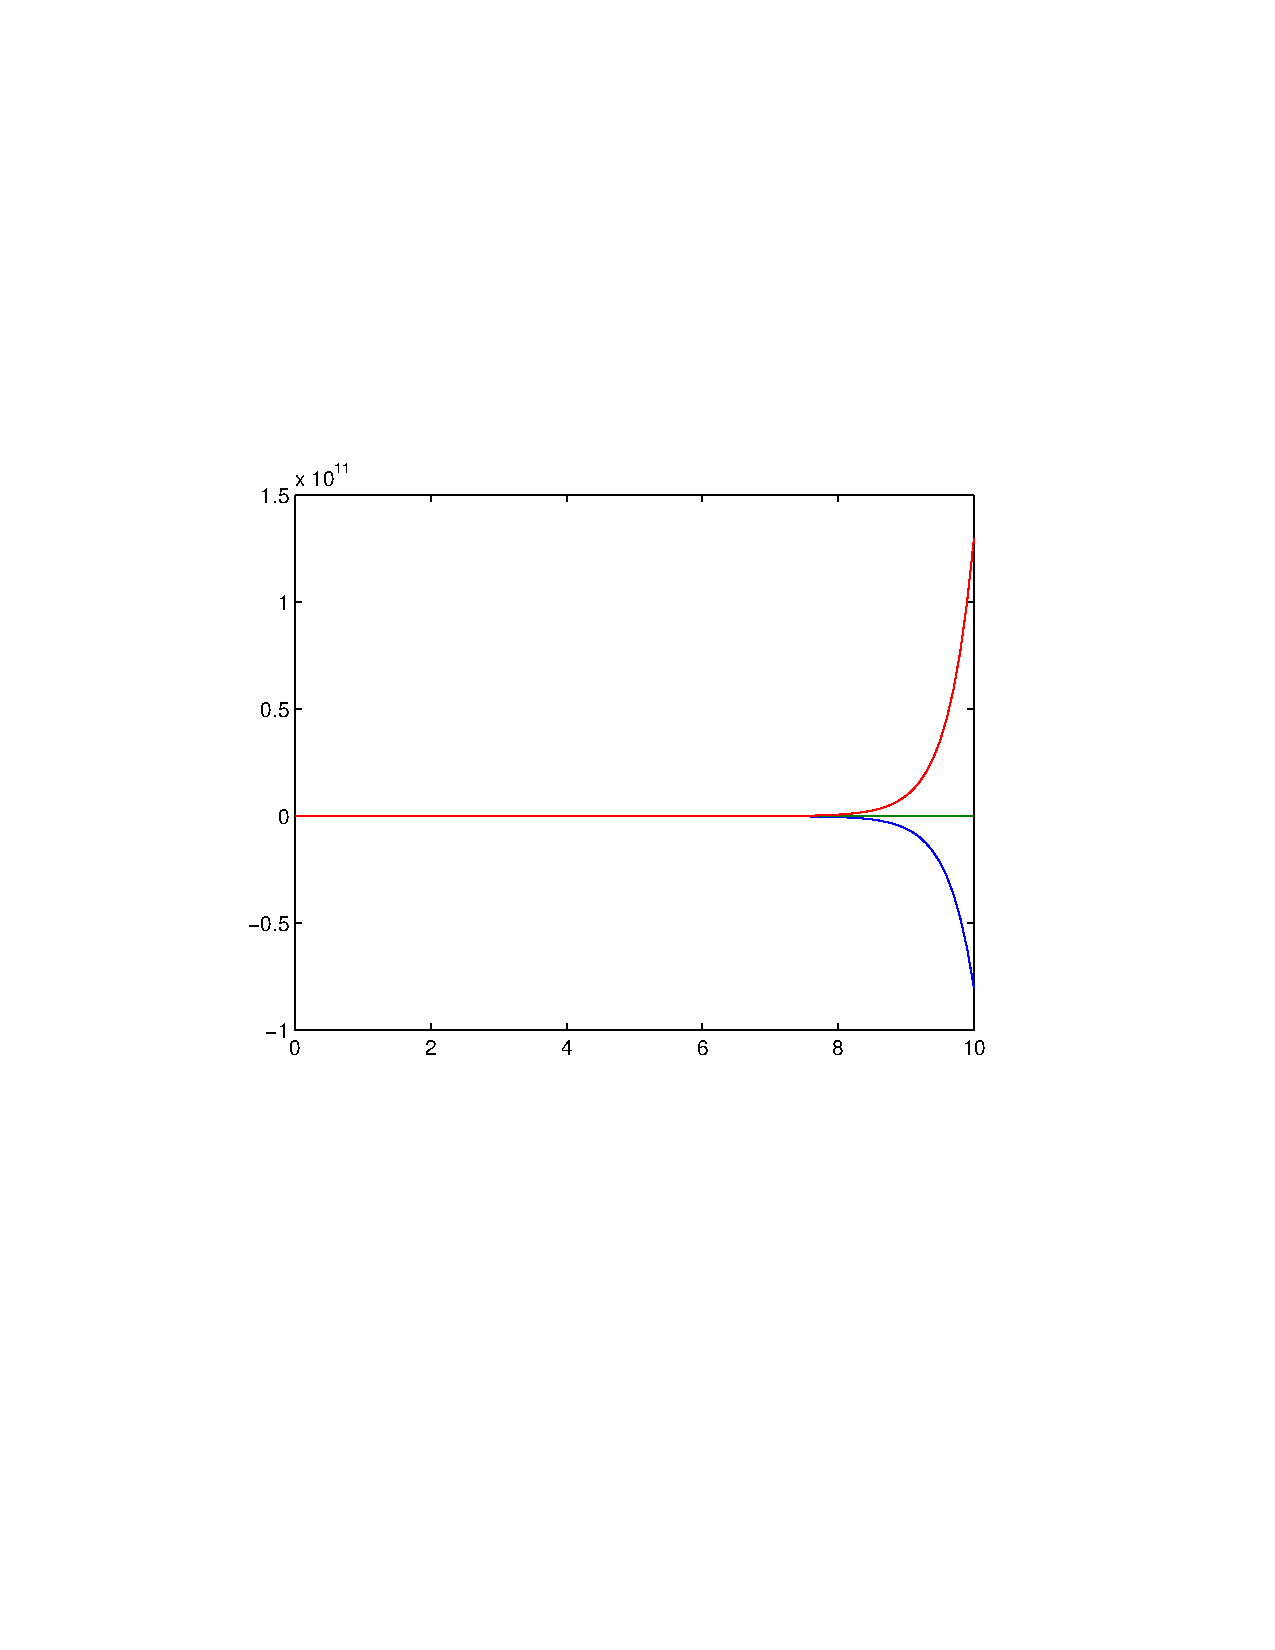
\includegraphics[width=\textwidth]{num2} 
\end{minipage}
\end{figure}
\end{document}
